\documentclass[tikz,border=8pt]{standalone}
% Shared look for every TikZ diagram. Load with \input{../../tools/tikz-style.tex}
\usepackage[T1]{fontenc}
\usepackage{lmodern}
\renewcommand{\sfdefault}{lmr}  % diagrams use the same serif as the text
\usetikzlibrary{arrows.meta, positioning, shapes.geometric, calc, fit, backgrounds}
\definecolor{cblue}{HTML}{4C78A8}
\definecolor{corange}{HTML}{F58518}
\definecolor{cgreen}{HTML}{54A24B}
\definecolor{cred}{HTML}{E45756}
\definecolor{cpurple}{HTML}{B279A2}
\definecolor{cgrey}{HTML}{6B6B6B}
\tikzset{
  every picture/.style={font=\sffamily, line width=1.2pt},
  box/.style={draw=#1, fill=#1!12, rounded corners=4pt, align=center, inner sep=7pt, minimum height=1.1cm},
  box/.default=cgrey,
  arrow/.style={-{Stealth[length=3mm]}, draw=cgrey, line width=1.4pt},
  title/.style={font=\sffamily\bfseries\Large},
  note/.style={font=\sffamily\small, text=cgrey, align=center},
}
\AtBeginDocument{\hyphenpenalty=10000 \exhyphenpenalty=10000}

\begin{document}
% The batch of section 3.3: three reviews, each a (time steps x 5) one-hot table, padded to 4 time steps -> (3, 4, 5).
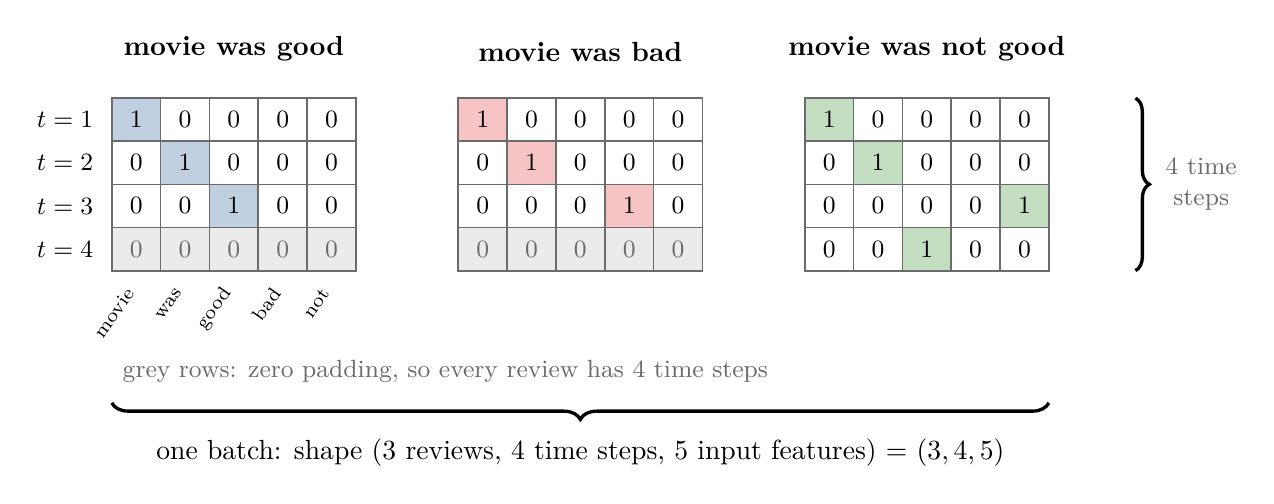
\begin{tikzpicture}[cell/.style={draw=cgrey, minimum width=0.62cm, minimum height=0.55cm, font=\sffamily\small, line width=0.6pt}]
  \newcommand{\review}[4]{% x offset, title, list of one-hot positions (0 = padding), colour
    \node[font=\sffamily\bfseries, anchor=south] at (#1+1.55, 0.05) {#2};
    \foreach \p [count=\r] in #3 {
      \foreach \c in {1,...,5} {
        \pgfmathparse{\p==\c ? "1" : "0"}\let\v\pgfmathresult
        \ifnum\p=0 \node[cell, fill=black!8, text=cgrey] at (#1+\c*0.62-0.31, -\r*0.55) {0};
        \else\ifnum\v=1 \node[cell, fill=#4!35] at (#1+\c*0.62-0.31, -\r*0.55) {1};
        \else \node[cell] at (#1+\c*0.62-0.31, -\r*0.55) {0};\fi\fi
      }
    }
  }
  \review{0}{movie was good}{{1,2,3,0}}{cblue}
  \review{4.4}{movie was bad}{{1,2,4,0}}{cred}
  \review{8.8}{movie was not good}{{1,2,5,3}}{cgreen}
  \foreach \t in {1,...,4} {\node[font=\sffamily\small, anchor=east] at (-0.1, -\t*0.55) {$t = \t$};}
  \foreach \w [count=\c] in {movie,was,good,bad,not} {\node[font=\sffamily\scriptsize, rotate=55, anchor=east] at (\c*0.62-0.31, -2.6) {\w};}
  \node[note, anchor=west] at (0, -3.75) {grey rows: zero padding, so every review has 4 time steps};
  \draw[decorate, decoration={brace, amplitude=6pt, mirror}] (0, -4.15) -- (11.9, -4.15)
    node[midway, below=9pt, font=\sffamily] {one batch: shape (3 reviews, 4 time steps, 5 input features) = $(3, 4, 5)$};
  \draw[decorate, decoration={brace, amplitude=5pt}] (13.0, -0.28) -- (13.0, -2.47) node[midway, right=7pt, note] {4 time\\steps};
\end{tikzpicture}
\end{document}
